\chapter{Preliminares}

En este capítulo se expone de manera breve la notación y algunas características de las distribuciones gaussiana, gaussiana $p$ variada, gamma, gamma inversa, Wishart, Wishart inversa, gaussiana inversa generalizada, gaussiana inversa, las cuales se usarán en capítulos posteriores.

La notación a emplear adoptará la usada en el enfoque bayesiano, para ser consistente
con el tipo de modelación que se realizará. Por lo que si la variable o vector aleatorio, $X$, tiene una función de densidad parametrizada por algún vector de parámetros, $\Theta$, entonces la función de densidad de $X$ se denotará por $f(X|\Theta)$, que se lee e interpreta como: $X$ se distribuye $f(x)$ dado $\Theta$. La función de densidad de $\Theta$ será $f(\Theta|\theta_{0})$ para algún vector de parámetros $\theta_{0}$. Esta función de densidad es conocida como distribución a priori, y se interpreta de la misma manera que la distribución de $X$, salvo que representa un grado subjetivo de creencia respecto a $\Theta$. Para la función de densidad de $\Theta$ condicionada en $X$ usaremos la notación $f(\Theta|X)$, la cual se conoce como densidad a posteriori (Bernardo $\&$ Smith, $2000$)\cite{}. 

\section{Distribución gaussiana}
Se dice que una variable aleatoria $X$, que toma valores en los números reales, se distribuye normal con media $\mu$, y desviación estándar $\sigma$, si su función de densidad de probabilidad es de la siguiente manera,

\begin{equation}
	f_{x}(x|\mu, \sigma)=\frac{1}{2\sqrt{\pi \sigma}}\exp^{-\frac{(x-\mu)^2}{2\sigma^2}}I_{(-\infty,\infty)}(x).
\end{equation}

En la distribución gaussiana, dos parámetros caracterizan la forma de la distribución,  $\mu=E[X]$, y $\sigma^2=Var[X]$, de aquí que el parámetro $\mu$ nos da información sobre la localización de la distribución, mientras que $\sigma$ de la dispersión.

Para referirnos a que $X$ se distribuye gaussiana con parámetros $\mu$ y $\sigma$, usaremos la notación, $X|\mu,\sigma$ se distribuye $N(x|\mu,\sigma)$.

Como se mencionó anteriormente, el parámetro $\mu$ es una medida de localización, mientras que el parámetro $\sigma$ es una medida de dispersión de la distribución gaussiana, lo cual se ilustra en las siguientes gráficas. En la gráfica \ref{fig:Ncambioenmedia} se pueden observar cuatro distribuciones gaussianas, etiquetadas como a), b), c) y d), con el mismo parámetro de dispersión $\sigma=1$, pero diferentes parámetros de localización, es decir,  $\mu_{1}=0$, $\mu_{2}=2$, $\mu_{3}=4$ y $\mu_{4}=6$ respectivamente.

\begin{figure}[h!]
	\centering
	%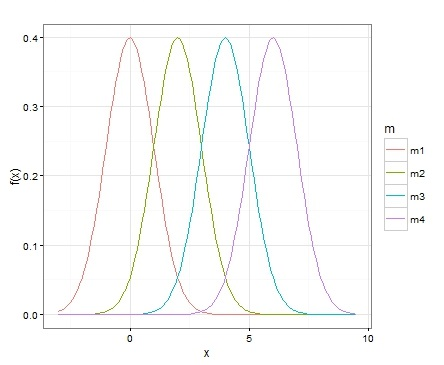
\includegraphics{Figuras/cambiosenmedia}
	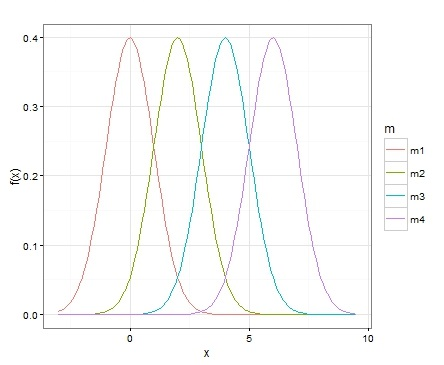
\includegraphics[width=.8\linewidth]{Figuras/cambiosenmedia.jpeg}
	\caption{Distribuciones gaussianas con el mismo par\'ametro de dispersi\'on, pero diferentes par\'ametros de localizaci\'on.}
	\label{fig:Ncambioenmedia}
\end{figure}

Por otro lado, en la gráfica \ref{fig:Ncambiosd}, se pueden observar cuatro distribuciones gaussianas, etiquetadas como a), b), c) y d), con parámetros de localización $\mu_{1}=0$, $\mu_{2}=0$, $\mu_{3}=0$ y $\mu_{4}=0$, y parámetros de dispersión $\sigma_{1}=0$, $\sigma_{2}=2$, $\sigma_{3}=4$ y $\sigma_{4}=6$, respectivamente; adviértase cómo incrementan las colas de la distribución gaussiana entre mayor es el parámetro de dispersión.

\begin{figure}[ht]
	\centering
	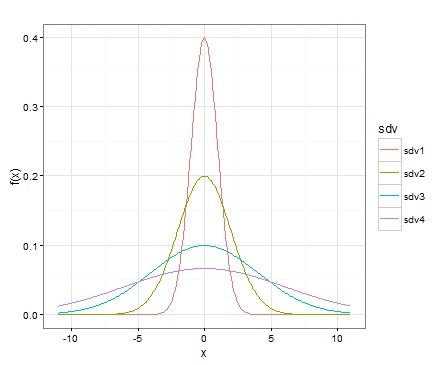
\includegraphics[width=.8\linewidth]{Figuras/cambiosd}
	\caption{Distribuciones gaussianas con diferente parámetro de dispersión.}
	\label{fig:Ncambiosd}
\end{figure}

\pagebreak

Como caso particular de la distribución gaussiana tenemos la distribución gaussiana estándar, que se obtiene cuando el parámetro $\mu =0$, y $\sigma=1$. También podemos llegar a esta distribución mediante un proceso de normalización de la distribución ($2.1$), es decir, si $X$ se distribuye  $N(x|\mu,\sigma)$, y si consideramos la transformación $Y=\frac{X-\mu}{\sigma}$, entonces $Y$ se distribuye $N(y|0,1)$.

Por último, la función generadora de momentos y característica de una distribución gaussiana es de la siguiente manera (Ross Shelder, Probability ),
\begin{equation}
	m_{x}(t)=\exp^{\sigma t+\frac{t\mu\sigma^2}{2}}
\end{equation}

\begin{equation}
	\Phi_{x}(it)=\exp \{\sigma it+\frac{it\mu\sigma^2}{2} \}
\end{equation}


\section{Distribución gaussiana p-variada}
Se dice que un vector aleatorio $X$ de dimensión $p$, con parámetros $\mu$ y $\Sigma$, que toma valores tanto positivos como negativos en cada entrada, tiene una distribución gaussiana $p$-variada  si su función de densidad es de la siguiente forma:
\begin{equation*}
	f_{x}(X|\mu,\Sigma)=\dfrac{1}{(2\Pi)^{p/2}|\Sigma|^{1/2}}exp\{-1/2(X-\mu)'\Sigma^{-1}(X-\mu)\}I_{R^{p}}(x),
\end{equation*}
donde $\mu=E[X]$, de dimensión $p$, es el vector de medias, y $\Sigma=Cov[X]$ de dimensión $p\times p$, matriz simétetrica positiva definida, es la matriz de varianza-covarianza. Análogamente a la distribución gaussiana, el vector $\mu$ es un vector de posición, el cual indica donde está centrada la distribución del vector aleatorio $X$. Mientras que la matriz $\Sigma$ está formada por las varianzas de cada $X_{i}$ en las entradas diagonales, es decir en la $(i,i)$ entrada, y por las covarianzas $Cov[X_{i,j}]$ en la $(i,j)$ entrada de la matriz. De aquí que la matriz de varianzas-covarianzas indique la dispersión del vector aleatorio $X$ alrededor del vector de medias $\mu$.

En este caso, si $X$ es un vector aleatorio de dimensión $p$, con vector de medias $\mu$, y matriz ve varianza-covarianza $\Sigma$, usaremos la notación $X$ se distribuye $N_{p}(x|\mu,\Sigma)$.

Como se mencionó anteriormente el vector $\mu$ es un parámetro de localización, de la distribución gaussiana $p$-variada, lo cual se ilustra a continuación para el caso bivariado. En la gráfica \ref{fig:NPM} se muestran  tres distribuciones gaussianas a), b) y c); todas con la misma matriz de varianza-covarianza $I$, con $\sigma_{1}=\sigma_{2}=1$ y $\sigma_{1,2}=0$; pero con vectores de medias $\mu_{1}=(-2,-2)$, $\mu_{2}=(0,0)$ y $\mu_{3}=(2,2)$, respectivamente. 

\begin{figure}[ht]
	\centering
	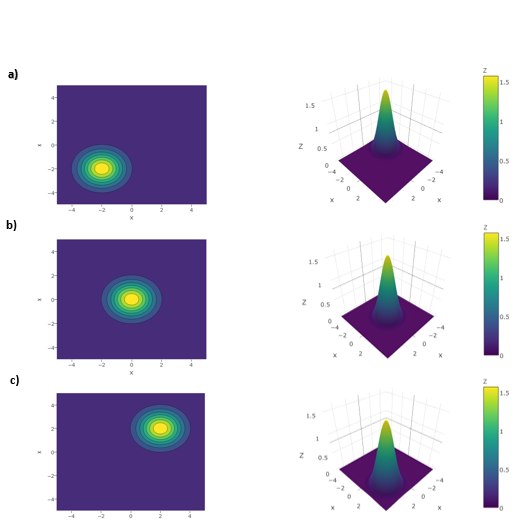
\includegraphics[width=.8\linewidth]{Figuras/NPM}
	\caption{Distribución gaussiana $p$-varaida con diferentes vectores de medias $\mu$.}
	\label{fig:NPM}
\end{figure}

\pagebreak
Ahora si nos enfocamos en la matriz de varianza-covarianza $\Sigma$, entre mayor sea la varianza del elemento $x_{i}$ del vector aleatorio $X$, mayor será la dispersión de la distribución de $X$ en el eje coordenado correspondiente a $x_{i}$.

Por otro lado, entre mayor o menor sea la covarianza entre algún par de elementos $x_{i}$ y $x_{j}$ pertenecientes a $X$, la distribución de $X$ tendrá una notable forma elíptica en los ejes cordenados $i$ y $j$, la cual está ligada a la interpretación de la correlación lineal entre $x_{i}$ y $x_{j}$, pues si $Cov[x_{i},x_{j}]$ es mayor a cero, la distribución de $X$ tendrá una foma elíptica centrada en el vector de medias $\mu$, pero rotada entre $0$ y $90$ grados, lo que indica que hay una dependencia lineal positiva entre el $i$-ésimo y $j$-ésimo elemento de $X$. Mientras que, sí la covarianza entre el $i$-ésimo y $j$-ésimo elemento de $X$ es menor a cero, la distribución de $X$ en los ejes coordenados $i$ y $j$ tendrá una forma elíptica rotada entre $90$ y $180$ grados. Los dos puntos anteriores se ilustran a cuntinuación para el caso bivariado.

En la gráfica \ref{fig:NPMsd} a) se observa una distribución gaussiana bivariada con vector de medias $\mu=(0,0)$, y con matriz de varianza-covarianza, $\Sigma$, con las entradas $Var[X]=1$, $Var[Y]=5$ y $Cov[X,Y]=0$. En b) con vector de medias $\mu=(0,0)$, $Var[X]=1$, $Var[Y]=1$ y $Cov[X,Y]=0$. Y en c) con vector de medias $\mu=(0,0)$, $Var[X]=5$, $Var[Y]=1$ y $Cov[X,Y]=0$. 

En la gráfica \ref{fig:NPcor} a) se observa una distribución gaussiana bivariada con vector de medias $\mu=(0,0)$, y con matriz de varianza-covarianza, $\Sigma$, con las entradas $Var[X]=2$, $Var[Y]=2$ y $Cov[X,Y]=0.75$. En b) con vector de medias $\mu=(0,0)$, $Var[X]=5$, $Var[Y]=5$ y $Cov[X,Y]=-0.75$. 

\begin{figure}[ht]
	\centering
	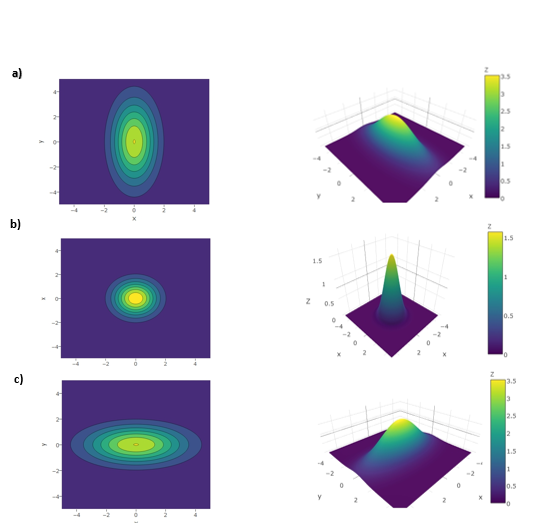
\includegraphics[width=.9\linewidth]{Figuras/NPMsd}
	\caption{Distribución gaussiana bivariada con diferentes varianzas y covarianzas}
	\label{fig:NPMsd}
\end{figure}

\begin{figure}[ht]
	\centering
	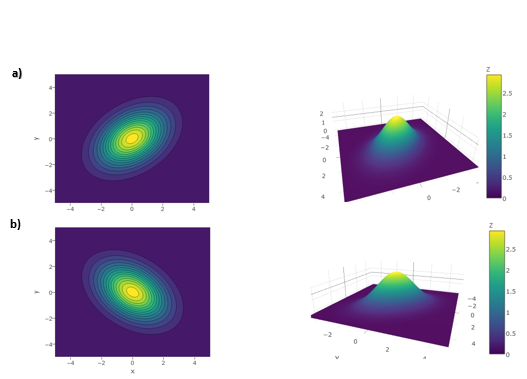
\includegraphics[width=.9\linewidth]{Figuras/NPcor}
	\caption{Distribución gaussiana bivariada con diferentes valores de covarianza }
	\label{fig:NPcor}
\end{figure}

\newpage
Análogamente a la distribución gaussiana estándar, si $X$ se distribuye $N_{p}(x|\mu,\Sigma)$, y para cada entrada $X_{i}$ del vector aleatorio $X$ consideramos la transformación $Y_{i}=\frac{X_{i}-\mu_{i}}{\sigma}$, entonces el vector aleatorio $Y$ resultante tendrá una distribución $N_{p}(x|$\boldmath$0$,\boldmath $I$), donde \boldmath$0$ es el vector cero de dimensión $p$, mientras que \boldmath $I$ es la matriz identidad de dimensión $p\times p$. A esta distribución se le conoce como gaussiana estándar $p$-variada.

Por último, la función generadora de momentos y característica de la distribución normal $p$-variada son las siguiente: 

\begin{equation}
	m_{x}(t)=\exp\{\mu t +\frac{\acute{t}\Sigma t}{2}\}
\end{equation}

\begin{equation}
	\Phi_{x}(it)=\exp\{\mu it -\frac{\acute{t}\Sigma t}{2}\}
\end{equation}

\section{Distribución gamma}
Se dice que una variable aleatoria $X$, que toma valores en los números reales positivos, se distribuye gamma con parámetros $\lambda$ y $\alpha$, si su función de densidad de probabilidad es de la siguiente manera:

\begin{equation}
	f_{x}(x|\lambda, \alpha)=\frac{\lambda^{\alpha}x^{\alpha-1}}{\gamma(\alpha)}\exp\{-\lambda x\}I_{(0,\infty)}(x)
\end{equation}

En la distribución gamma dos parámetros caracterizan la forma de la distribución,  $\lambda$ y $\gamma$. El parámetro $\lambda$ toma valores mayores a cero, mientras que $\alpha$ puede tomar valores mayores o iguales a cero. El parámetro $\lambda$ también es conocido como parámetro de escala e influye en el tamaño de la densidad respecto al eje $y$. Por otro lado, el parámetro $\alpha$ influye en la forma de la distribución. 

Para referirnos a que $X$ se distribuye gamma con parámetros $\lambda$ y $\alpha$, usaremos la notación $X|\lambda,\alpha$ se distribuye $\Gamma(x|\lambda,\alpha)$.

Como se mencionó anteriormente, el parámetro $\lambda$ es un parámetro de escala, mientras que el parámetro $\alpha$ es un parámetro de forma, lo cual se ilustra a continuación.

En la gráfica \ref{fig:gammadifernetelambda} se muestran cuatro distribuciones gamma con el mismo parámetro forma $\alpha=1$, pero con distintos parámetros de escala, es decir, con $\lambda_{1}=1$, $\lambda_{2}=2$, $\lambda_{3}=3$ y $\lambda_{4}=4$, respectivamente. 
\begin{figure}[ht]
	\centering
	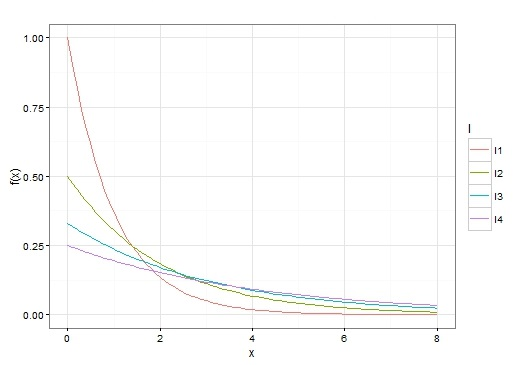
\includegraphics[width=0.85\linewidth]{Figuras/gammadifernetelambda}
	\caption{Distribución gamma con diferente parámetro $\lambda$}
	\label{fig:gammadifernetelambda}
\end{figure}

En la gráfica \ref{fig:gammaalfa} se muestran cuatro distribuciones gamma con al mismo parámetro de escala $\lambda=1$, pero con distintos parámetros de forma, es decir, con $\alpha_{1}=1$, $\alpha_{2}=2$, $\alpha_{3}=3$ y $\alpha_{4}=4$, respectivamente. Adviertase que conforme $\alpha$ es menor el sesgo de la distribución aumenta a la derecha, mientras que si es menor disminuye a la derecha y aumenta a la izquierda. 

\pagebreak

\begin{figure}
	\centering
	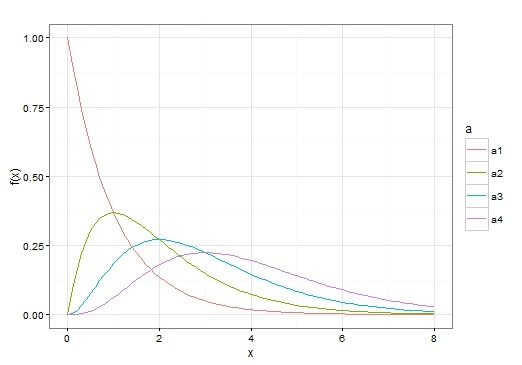
\includegraphics[width=0.8\linewidth]{Figuras/gammaalfa}
	\caption{Distribución gamma con diferente parámetro $\alpha$}
	\label{fig:gammaalfa}
\end{figure}

Si la variable aleatoria $X$ se distribuye gamma con parámetros $\lambda$, $\alpha$, entonces:
%\begin{enumerate}
%	\item \begin{equation*}
%	E[x]=\frac{\alpha}{\lambda}
%	\end{equation*}
%	\item \begin{equation*}
%	Var[x]=\frac{\alpha}{\lambda^{2}}
%	\end{equation*}
%	\item \begin{equation*}
%	m_{x}(t)=(\frac{\lambda}{\lambda-t})^{\alpha}
%	\end{equation*}
%	\item \begin{equation*}
%	\Phi_{x}(it)=(\frac{\lambda}{\lambda-it})^{\alpha}
%	\end{equation*}
%\end{enumerate}
\begin{eqnarray}
	E[x]&=&\frac{\alpha}{\lambda}, \nonumber\\
	Var[x]&=&\frac{\alpha}{\lambda^{2}}, \nonumber\\
	m_{x}(t)&=&(\frac{\lambda}{\lambda-t})^{\alpha},\nonumber\\
	\Phi_{x}(it)&=&(\frac{\lambda}{\lambda-it})^{\alpha}, \nonumber\\
\end{eqnarray}

Por último, es importante mencionar que la distribución gamma es la distribución a priori conjugada de la distribución wishart, la cual se intruduce más adelante.

\section{Distribución gamma inversa}

La distribución gamma inversa resulta de aplicar la transformación $X=\frac{1}{y}$ a la variable aleatoria $Y$, donde $Y$ se distribuye gamma con parámetros $\lambda$ y $\alpha$. Dicho lo anterior se tiene la siguiente definición.

Se dice que una variable aleatoria $X$, que toma valores en los números reales positivos, se distribuye gamma inversa con parámetros $\lambda$ y $\alpha$, si su función de densidad de probabilidad es de la siguiente manera:

\begin{equation}
	f_{x}(x|\lambda, \alpha)=\frac{\lambda^{\alpha}x^{1-\alpha}}{\gamma(\alpha)}\exp\{-\frac{\lambda}{x}\}I_{(0,\infty)}(x).
\end{equation}

La distribución gamma inversa hereda sus dos parámetros de la distribución gamma, por lo que tanto $\lambda$ como $\alpha$ tienen las mismas restricciones que en la distribución gamma, y también caracterizan la forma de la distribución. Al igual que en la distribución gamma, el parámetro $\lambda$ es conocido como parámetro de escala e influye en el tamaño de la densidad respecto al eje $y$. Mientras que el parámetro $\alpha$ influye en la forma de la distribución. 

Para referirnos a que $X$ se distribuye gamma inversa con parámetros $\lambda$ y $\alpha$, usaremos la notación $X|\lambda,\alpha$ se distribuye $\Gamma Inv(x|\lambda,\alpha)$.

Como se mencionó anteriormente, el parámetro $\lambda$ es un parámetro de escala, mientras que el parámetro $\alpha$ es un parámetro de forma, lo cual se ilustra a continuación.

En la gráfica \ref{fig:invgammalambda} se muestran cuatro distribuciones gamma inversa con el mismo parámetro de forma $\alpha=1$, pero con distintos parámetros de escala, es decir, con $\lambda_{1}=1$, $\lambda_{2}=2$, $\lambda_{3}=3$ y $\lambda_{4}=4$, respectivamente. 

\begin{figure}[ht]
	\centering
	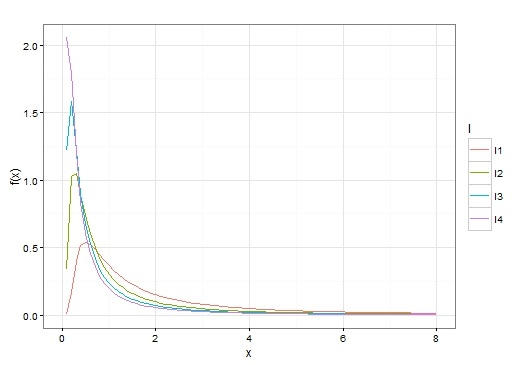
\includegraphics[width=1\linewidth]{Figuras/invgammalambda}
	\caption{Distribución gamma inversa con diferente parámetro $\lambda$}
	\label{fig:invgammalambda}
\end{figure}

En la gráfica \ref{fig:invgammaalfa} se muestran cuatro distribuciones gamma inversa con al mismo parámetro de escala $\lambda=1$, pero con distintos parámetros de forma, es decir, con $\alpha_{1}=1$, $\alpha_{2}=2$, $\alpha_{3}=3$ y $\alpha_{4}=4$, respectivamente. Adviertase que conforme $\alpha$ es menor la curtosis de la distribución aumenta, mientras que si es mayor disminuye.

\newpage
\begin{figure}[ht]
	\centering
	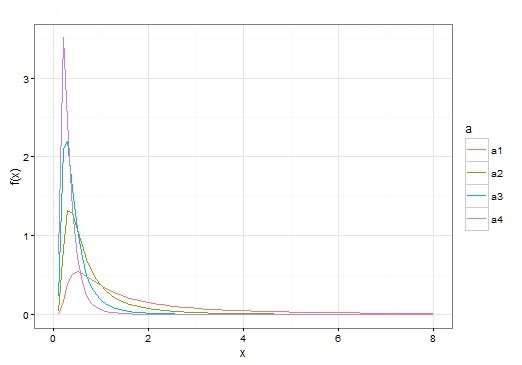
\includegraphics[width=0.9\linewidth]{Figuras/invgammaalfa}
	\caption{Distribución gamma inversa con diferente parámetro $\alpha$}
	\label{fig:invgammaalfa}
\end{figure}


Si la variable aleatoria $X$ se distribuye gamma inversa con parámetros $\lambda$, $\alpha$, entonces:
% \begin{enumerate}
%	\item \begin{equation*}
%	E[x]=\frac{\alpha}{\alpha - 1}
%	\end{equation*}
%	\item \begin{equation*}
%	Var[x]=\frac{\lambda^{2}}{(\alpha-1)^{2}(\alpha-1)}
%	\end{equation*}
%	\item \begin{equation*}
%	\Phi_{x}(it)=(\frac{2(-\lambda it)^{\alpha/2}}{\gamma (\alpha)})\kappa(\sqrt{-4\lambda it})
%	\end{equation*}

%\end{enumerate}
\begin{eqnarray}
	E[x]&=&\frac{\alpha}{\alpha - 1}, \nonumber\\
	Var[x]&=&\frac{\lambda^{2}}{(\alpha-1)^{2}(\alpha-1)},\nonumber\\
	\Phi_{x}(it)&=&(\frac{2(-\lambda it)^{\alpha/2}}{\gamma (\alpha)})\kappa(\sqrt{-4\lambda it}),\nonumber\\
\end{eqnarray}

Por último, es importante mencionar que la distribución Gamma Inversa es la distribución apriori conjugada de la distribución Wishart Inversa, la cual se intruduce más adelante.

\pagebreak
\section{Distribución Wishart}

La distribución whishart es utilizada como distribución de la matriz de varianza-covarianza de
vectores aleatorios normales de dimensión $p$, y se deriva de la siguiente manera:

Supongamos que tenemos $n$ vectores aleatorios $X$  de dimensión $p$ que se distribuyen $N_{p}(X|0,\Sigma)$, luego un estimador de la matriz de varianza-covarianza es $S=\Sigma_{i=1}^{n}x_{i}x_{i}/n$, que es una matriz positiva y simétrica de dimensión $p\times p$, por lo que para los distintos valores que tomen los vectores aleatorios $X$, $S$ también tomará un valor diferente, por lo que es natural preguntarse por la distribución de $S$, con lo cual se llega a la siguiente caracterización. 

Se dice que una matriz $S$ de dimensión $pxp$, simétrica y positiva definida, se distribuye wishart con $n$ grados de libertad, si su densidad es de la siguiente forma:
\begin{equation*}
	f_{S}(S|\Sigma,n,p)= c\frac{|S|^{(n-p-1)/2}}{|\Sigma|^{n/2}}\exp(-\frac{1}{2}tr(\Sigma^{-1}S)),
\end{equation*}

donde $c=\left(2^{np/2}\pi ^{p(p-1)/4}\prod_{i=1}^{p}\gamma(\dfrac{n+1-i}{2})\right)^{-1}$, $\Sigma$ es una matriz simétrica y positiva definida de dimensión $pxp$, y se le conoce como matriz de escala, $n$ es elnúmero de vectores disponibles, y es mayor a la dimensión de los vectores, es decir, mayor que $p$. En este caso usaremos la notación $S$ se distribuye $W(S|\Sigma,n,p)$.\\

Algunas características numéricas de la distribución Whisart son las siguientes:

%\begin{enumerate}
%\item 
\begin{equation*}
	E[S]=p\Sigma,
\end{equation*} \nonumber\\
%\item 
La distribución marginal del $i$-ésimo componente de la distribución wishart se distribuye $\Gamma$($\frac{1}{2}$,$\frac{1}{2}$).\nonumber

%\end{enumerate}




\section{Distribución Wishart inversa}
Se dice que una matriz $G$ de dimensión $p \times p$, simétrica y positiva definida, se distribuye wishart inversa con $n$ grados de libertad, si su función de densidad es de la siguiente forma:
\begin{equation*}
	f_{G}(G)=c\frac{|K|^{(n-p-1)/2}}{|G|^{n/2}}\exp(-\frac{1}{2}tr(G^{-1}K)),
\end{equation*}
donde $c=\left(2^{(n-p-1)p/2}\pi^{p(p-1)/4}\prod_{i=1}^{p}\gamma(\frac{n-p-i}{2})\right)^{-1}$, $K$ es una matriz simétrica y definida positiva, y se le conoce como matriz de escala. En este caso usaremos la notación $G$ se distribuye $W^{-1}(G|K,n,p)$.\\

Una propiedad importante que liga a la distribución wishart y wishart inversa, es la siguiente.\\ 

Si una matriz aleatoria $\Sigma$ de dimensión $p\times p$ se distribuye whisart con matriz de escala $S$, y con $n$ grados de libertad, entonces su matriz inversa, $\Sigma^{-1}$, se distribuye whisart inversa con matriz de escala $S^{-1}$, y con $n+p+1$ grados de libertad.

\section{Distribución gaussiana inversa generalizada}
Se dice que la variable aleatori $X$, que toma valores en los números reales positivos, tiene una distribución gaussiana inversa generalizada, denotada por $GIG(x|\lambda,\xi,\Psi)$, si su densidad es de la siguiente forma:

\begin{equation*}
	f(x)= \dfrac{\xi^{-\lambda}\sqrt{\xi\Psi}^{\lambda}x^{\lambda-1}\exp{\frac{-1}{2}(\xi x^{-1} + \Psi x)}}{2\kappa_{\lambda}(\sqrt{\xi\Psi})}I_{(0,\infty)}(x),  
\end{equation*}
donde $\kappa_{\lambda(.)}$ es una función modificada de Bessel de tercer tipo, y si $\lambda<0$, entonces $\xi>0$, $\Psi \ge 0 $; si $\lambda=0$, entonces $\xi>0$, $\Psi > 0 $, si $\lambda>0$, entonces $\xi\ge 0$, $\Psi > 0 $.\\

En la distribución gaussiana inversa generalizada tres parámetros caracterizan la forma de la distribución. Tanto el parámetro $\xi$ como el parámetro $\Psi$ influyen en la escala de la distribución, mientras que el parámetro $\lambda$ en la forma. El punto anterior se ilustra a continuación.\\

En la gráfica \ref{fig:gigdiferentesvaloresdepsi} se muestran cuatro distribuciones GIG, todas con los mismos parámetros $\lambda=1$ y $\xi=1$, pero con diferentes parámetros $\psi_{1}=0.5$, $\psi_{2}=1$, $\psi_{3}=2$ y $\psi_{4}=4$, respectivamente. Es importante notar que entre menor es el valor de $\psi$, mayor es la curtosis de la distribución. \\


\begin{figure}[ht]
	\centering
	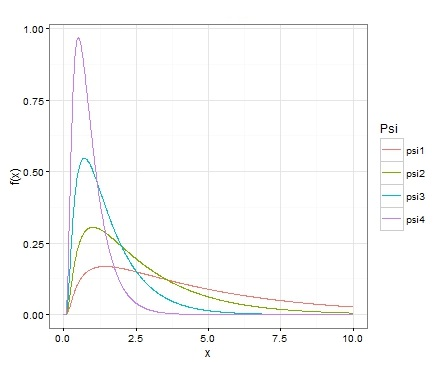
\includegraphics[width=0.8\linewidth]{Figuras/gigdiferentesvaloresdepsi}
	\caption{Distribución GIG con diferentes valores del parámetro $\psi$.}
	\label{fig:gigdiferentesvaloresdepsi}
\end{figure}

En la gráfica \ref{fig:gigcondiferentesvaloresdexi} se observan cuatro distribuciones GIG, todas con paámetros $\lambda=1$ , $\psi=1$, pero con diferentes parámetros $\xi_{1}=0.5$, $\xi_{2}=1$, $\xi_{3}=2$ y $\xi_{4}=4$, respectivamente. Es importante notar que entre mayor es el valor del parámetro $\xi$, mayor es el sesgo a la derecha de la distribución.

\newpage
\begin{figure}[ht]
	\centering
	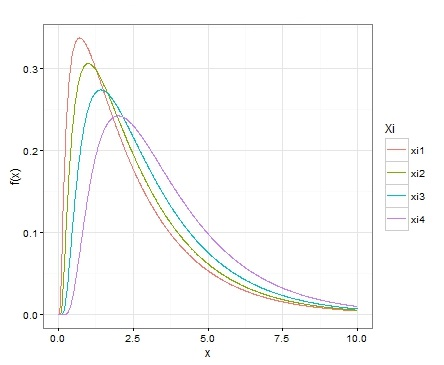
\includegraphics[width=0.8\linewidth]{Figuras/gigcondiferentesvaloresdexi}
	\caption{Distribución GIG con diferentes valores del parámetro $\xi$}
	\label{fig:gigcondiferentesvaloresdexi}
\end{figure}

En la gráfica \ref{fig:gigdiferentesvaloreslambda} se observan cuatro distribuciones GIG, todas con parámetros $\psi=1$ , $\xi=1$, pero con diferentes parámetros $\lambda_{1}=-0.5$, $\lambda_{2}=0$, $\lambda_{3}=.5$ y $\lambda_{4}=1$, respectivamente. En este caso el parámetro $\lambda$ también influye en la curtosis de la distribución, ero sobre todo influye en la cola de esta. También el parámetro $\lambda$ influye en la failia paramétrica, pues si la variable aleatoria $X$ se distribuye GIG, con parámetro $\lambda=0$ entonces se obtiene la distribución hiperbólica, mientras que si $\lambda=-0.5$ se obtiene la distribución Gaussiana Inversa de la cual se hablará posteriormente. 

\newpage 
\begin{figure}[ht]
	\centering
	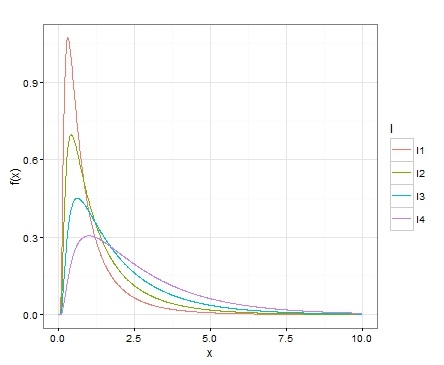
\includegraphics[width=0.8\linewidth]{Figuras/gigdiferentesvaloreslambda}
	\caption{Distribución GIG con diferentes valores de $\lambda$}
	\label{fig:gigdiferentesvaloreslambda}
\end{figure}


Ahora veamos algunos resultados de la distribución GIG. Si $X$ se distribuye $N\tilde{}(x|\lambda,\xi,\Phi)$, entonces su función generadora de momentos es:

\begin{eqnarray*}
\Phi (it) & = &\underset{-\infty }{\overset{\infty }{\int }}\exp(itx){\dfrac{\xi^{-\lambda}\sqrt{\xi\Psi}^{\lambda}x^{\lambda-1}\exp{\frac{-1}{2}(\xi x^{-1} + \Psi x)}}{2\kappa_{\lambda}(\sqrt{\xi\Psi})}}dx\\
 &=& c\underset{-\infty }{\overset{\infty }{\int }}\xi^{-\lambda}\frac{\sqrt{\xi(2it + \Psi)}^{\lambda}}{2\kappa_{\lambda}(\sqrt{\xi(2it + \Psi)})}\exp{\frac{-1}{2}(\xi x^{-1} + (2it+\Psi) x)}dx,\\ 
\end{eqnarray*}

con $c=\frac{\sqrt{\xi\Psi}^{\lambda}}{2\kappa_{\lambda}(\sqrt{\xi\Psi})}\frac{2\kappa_{\lambda}(\sqrt{\xi(2it + \Psi)})}{\sqrt{\xi(2it + \Psi)}^{\lambda}}$. La última integral vale uno por ser una densidad $N\bar{}(\lambda,\xi,2it + \psi)$ integrada sobre su soporte, por lo que:

\begin{equation*}
	\Phi(it)=\frac{\sqrt{\xi\Psi}^{\lambda}}{\kappa_{\lambda}(\sqrt{\xi\Psi})}\frac{\kappa_{\lambda}(\sqrt{\xi(2it + \Psi)})}{\sqrt{\xi(2it + \Psi)}^{\lambda}}.
\end{equation*}

Si $X$ se distribuye $N\tilde{}(x|\lambda,\xi,\Phi)$, entonces su $r$-ésimo momento es:
\begin{equation*}
	E[X^{r}]=\underset{-\infty }{\overset{\infty }{\int }}x^{r}\dfrac{\xi^{-\lambda}\sqrt{\xi\Psi}^{\lambda}x^{\lambda-1}\exp{\frac{-1}{2}(\xi x^{-1} + \Psi x)}}{2\kappa_{\lambda}(\sqrt{\xi\Psi})}dx
\end{equation*}
\begin{equation*}
	=\frac{x^{r}2\kappa_{\lambda+r}(\sqrt{\xi\Psi})}{\sqrt{\xi\Psi}^{r}2\kappa_{\lambda}(\sqrt{\xi\Psi})}\underset{-\infty }{\overset{\infty }{\int }}\dfrac{\xi^{-\lambda-r}\sqrt{\xi\Psi}^{\lambda+r}x^{\lambda+r-1}\exp^{{\frac{-1}{2}(\xi x^{-1} + \Psi x)}}}{2\kappa_{\lambda+r}(\sqrt{\xi\Psi})}dx
\end{equation*}
Por lo tanto:
\begin{equation*}
	E[X^{r}]=(\frac{\xi}{\Psi})^{\frac{r}{2}}\frac{\kappa_{\lambda+r}(\sqrt{\xi \Psi})}{\sqrt{\kappa_{\lambda}(\sqrt{\xi\Psi})}}
\end{equation*}

\section{Distribución gaussiana inversa}
Se dice que la variable aleatoria $X$ tiene una distribución gaussiana inversa si su función de densidad es de la siguiente forma:
\begin{equation*}
	f_{x}(X|\lambda,\psi)=\sqrt{\dfrac{\lambda}{2\pi x^{3}}}\exp(-\dfrac{\lambda(x-\Psi)^{2}}{2\Psi^{2}x}),
\end{equation*}
para $\lambda$, $\psi$ y $X$ mayores a cero.
Como notación, si X se distribuye gausiana inversa con parámetros $\lambda$, $\Psi$, diremos que $X|\lambda,\psi$ se distribuye $GI(X|\lambda,\Psi)$.

Ahora veamos como es la función característica de esta distribución.
Si $X$ se distribuye $GI(x|\lambda,\Psi)$, entonces su función característica es:

\begin{equation}
	\begin{split} \label{211}
		\Phi_{x}(it)& =\int_{0}^{\infty}\exp^{itx}\sqrt{\dfrac{\lambda}{2\pi x^{3}}}\exp^{-\dfrac{\lambda(x-\Psi)^{2}}{2\Psi^{2}x}}dx\\
		&=\int_{0}^{\infty}\sqrt{\dfrac{\lambda}{2\pi x^{3}}}\exp(-\dfrac{\lambda}{2\Psi^{2}}(x-2\Psi-(itx2\Psi^{2}/\lambda)+\Psi^{2}x))dx\\
	\end{split}
\end{equation}
Trabajando únicamente con el exponente de la expresión anterior, y factorizando el término
$(1-\frac{it2\Psi^{2}}{\lambda})$ tenemo que:
\begin{equation} \label{212}
	\begin{split}
		%-\dfrac{\lambda}{2\Psi^{2}}(x-2\Psi-(itx2\Psi^{2}/\lambda)+\Psi^{2}x)  =
		&-\frac{\lambda}{2\Psi^{2}}(1-\frac{it2\Psi^{2}}{\lambda})
		(x-2\Psi/(1-\frac{it2\Psi^{2}}{\lambda})
		+\Psi^{2}/(1-\frac{it2\Psi^{2}}\lambda)\\ 
		&=-\dfrac{\lambda}{2\Psi^{2}}(1-\frac{it2\Psi^{2}}{\lambda})(x-2\Psi/(1-\frac{it2\Psi^{2}}{\lambda})
		+\Psi^{2}/x(1-\frac{it2\Psi^{2}}{\lambda})\\
		&+2\Psi/\sqrt{1-\frac{it2\Psi^{2}}{\lambda}}
		-2\Psi/\sqrt{1-\frac{it2\Psi^{2}}{\lambda}})\\
		&=\frac{\lambda}{\Psi}-\frac{\lambda}{\Psi}\sqrt{(1-\frac{it2\Psi^{2}}{\lambda})}-
		\frac{\lambda}{2x\Psi^{2}}(1-\frac{it2\Psi^{2}}{\lambda})(x
		-\Psi/\sqrt{1-2it\Psi^{2}/\lambda})^{2}
	\end{split}
\end{equation}

Por lo que la función característica queda de la siguiente forma:
\begin{eqnarray*}
\Phi_{x}(it) & =& (\exp^{\frac{\lambda}{\Psi}-\frac{\lambda}{\Psi}\sqrt{(1-\frac{it2\Psi^{2}}{\lambda})}}) \\
& &(\int_{0}^{\infty}\sqrt{\dfrac{\lambda}{2\pi x^{3}}}\exp^{\frac{\lambda}{2x\Psi^{2}}(1-\frac{it2\Psi^{2}}{\lambda})(x
	-\Psi/\sqrt{1-2it\Psi^{2}/\lambda})^{2}}dx)\\
&=&\exp(\frac{\lambda}{\Psi}-\frac{\lambda}{\Psi}\sqrt{(1-\frac{it2\Psi^{2}}{\lambda})})\\
\end{eqnarray*}


%\begin{equation}
%	\begin{split} \label{213}
%		\Phi_{x}(it)& =\exp^{\frac{\lambda}{\Psi}-\frac{\lambda}{\Psi}\sqrt{(1-\frac{it2\Psi^{2}}{\lambda})}} \int_{0}^{\infty}\sqrt{\dfrac{\lambda}{2\pi x^{3}}}\exp^{\frac{\lambda}{2x\Psi^{2}}(1-\frac{it2\Psi^{2}}{\lambda})(x
			%-\Psi/\sqrt{1-2it\Psi^{2}/\lambda})^{2}}dx\\
		%&=\exp^{\frac{\lambda}{\Psi}-\frac{\lambda}{\Psi}\sqrt{(1-\frac{it2\Psi^{2}}{\lambda})}}
	%\end{split}
%\end{equation}

El resultado anterior se sigue de que la integral previa es una distribución Gaussiana Inversa con parámetros $\lambda$, $\Psi/\sqrt{1-(2it\Psi^{2})/\lambda}$ integrada sobre su soporte, por lo cual vale $1$, y por lo tanto:
\begin{equation}
	\Phi_{x}(it)=\exp^{\frac{\lambda}{\Psi}-\frac{\lambda}{\Psi}\sqrt{(1-\frac{2it\Psi^{2}}{\lambda})}}
\end{equation}

Con el resultado anterior se puede probar que si $X$ se distribuye $GI(x|\lambda,\Psi)$, entonces:
%\begin{enumerate}
%	\item \begin{equation*}
%m_{x}(t)=\exp^{\frac{\lambda}{\Psi}-\frac{\lambda}{\Psi}\sqrt{(1-\frac{2t\Psi^{2}}{\lambda})}}
%\end{equation*}
%\item \begin{equation*}
%E[X]=\Psi
%\end{equation*}
%\item \begin{equation*}
%Var[X]=\frac{\Psi^{3}}{3}
%\end{equation*}
%\item \begin{equation*}
%Sesgo[X]=\frac{2\Psi^{4}}{\lambda}+\frac{3\Psi^{5}}{\lambda^{2}}
%\end{equation*}
%\end{enumerate}
\begin{eqnarray}
	m_{x}(t)= \exp^{\frac{\lambda}{\Psi}-\frac{\lambda}{\Psi}\sqrt{(1-\frac{2t\Psi^{2}}{\lambda})}},
	&&
	E[X]=\Psi,
	\nonumber\\
	Var[X]=\frac{\Psi^{3}}{3},
	&&
	Sesgo[X]=\frac{2\Psi^{4}}{\lambda}+\frac{3\Psi^{5}}{\lambda^{2}}.
	\nonumber
\end{eqnarray}

Entoces, al igual que la distibución gaussiana, la distribución gaussiana inversa tiene un parámetro de localización, es decir, $\Psi$. Es importante notar como afecta el parámetro $\lambda$ a la dispersión de la variable aleatpria $X$, y además, esta distribución siempre tiene un sesgo positivo ya que $\Psi$ y $\lambda$ son mayores a cero. Por lo que para valores muy pequeños de $\lambda$ o muy grandes de $\Psi$ la distribución tendrá más peso en la cola. 

%\citep{Abadie_DifferencesinDifferences}

%\citeauthor{AbadieGardeazabal_EconCostConflict}

%\citeyear{Abadie_etal_SyntheticControlComparative}

%\begin{figure}[htbp]
%	\centering
%	\caption{Una gr\'afica....}
%	\label{fig_ejemplo}
%		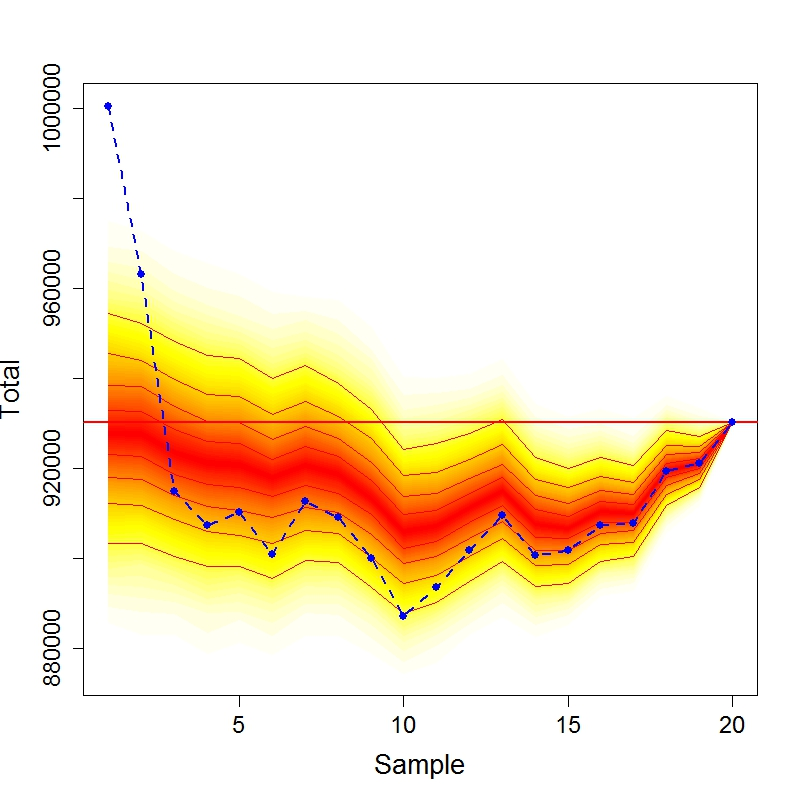
\includegraphics[width=0.97\textwidth]{Figuras/Ejemplo_Figura.jpg}
%\end{figure}

%
%	Table 1.
%
%\begin{table}[H]
%\begin{center}
%\begin{threeparttable}
%	\caption{Una tabla}
%	\label{tab_ejemplo}
%	{\scriptsize
%	\begin{tabular}{l c c c c c c c c c}
%		\toprule
%		\hline
%										& \multicolumn{9}{c}{Year}  \\
%		State		 			& 2003	& 2004	& 2005	& 2006	& 2007	& 2008	& 2009	& 2010	& 2011 \\
%		\midrule
%		\hline
%		\hline
%		Uno 		& 1.1	& 1.0	& 1.0	& 1.1	& 1.1	& 1.0	& 1.1	& 1.1	& 1.1 \\
%		Dos 		& 3.0	& 3.0	& 3.0	& 3.0	& 2.9	& 2.8	& 2.8	& 2.7	& 2.7 \\
%		\bottomrule
%		\hline
%	\end{tabular}
%	\begin{tablenotes}
%		\tiny
%		\item Source: ...
%		\item Note: ...
%	\end{tablenotes}
%	}			
%\end{threeparttable}
%\end{center}
%\end{table}